\documentclass[10pt,oneside,a4paper]{book} % Type de document
\usepackage[a4paper,margin=2cm,footskip=1cm,top=1cm]{geometry}	%Ajustement des marges
\usepackage[french]{babel} % Pour adopter les règles de typographie française
\usepackage[utf8]{inputenc} % Prévenir LaTeX de l'encodage
\usepackage{listings}	%permet de mettre des balise de code
\usepackage{hyperref}

\lstset{
           literate=
           {à}{{\`a}}1
           {é}{{\'e}}1
           {è}{{\`e}}1
           {ù}{{\`u}}1% etc, etc, etc
}			%resoud un problème d'encodage dans les balise de code

\usepackage{xcolor}	%couleur
\usepackage{graphicx}

%definition de macro pour les couleur
\definecolor{Zgris}{gray}{0.95}
\definecolor{CommentaireGris}{gray}{0.50}

\hypersetup{
colorlinks=true,
linkcolor=black,
urlcolor=black
}


\pagestyle{plain}

\title{\textbf{La Business Intelligence}}        % Titre du document
\author{Morgan JOUARD 
		\and
		Claude MICHEL 
		\and
		Jean-François ERLEM 
		\and
		Andre PONNOURADJANE 
}                                % Auteur
\date{26/05/2015}                            % Date de cr ́eation
 
\begin{document}                             % D ́ebut du document
\frontmatter				%hierarchie d'un ebook
\maketitle                              % G ́en ́eration du titre




\tableofcontents		%table des matieres


\chapter*{			%chapitre (* pour qu'il n'aparaisse pas dans la table des matieres)
Préface				
\vspace{3pt}\hrule\vspace{6pt}	%Trait e dessous du titre
} 
Ce livre est destinné au débutant....

\chapter*{
Introduction
\vspace{3pt}\hrule\vspace{6pt}
}
Il est tant de commencer a écrire notre livre....

\mainmatter			%partie principal du livre
\part{BI - La théorie}		%partie 1

\chapter[Business Inteligence]{
Business Inteligence
\vspace{3pt}\hrule\vspace{6pt}
} 
\section{Definition}		
\section{Principe}

\chapter[ETL]{
ETL
\vspace{3pt}\hrule\vspace{6pt}
} 
\section{Definition}
\subsubsection{ETL : Extract, Transform and Load}
Technologie informatique permettant d'effectuer des synchronisations massives d'informations d'une banque de données vers une autre.

\section{Principe}
Le principe de l'ETL est de permetre l’intégration et la consolidation de données de tous
types à l’aide des trois opérations suivantes:
\begin{itemize}		%indentation
  \item Extraction : \hfill \\
  			Identifier et extraire les données de sources ayant subi une modification depuis la dernière exécution.
  \item Transformation : \hfill \\
  			Appliquer diverses transformations aux données pour les nettoyer, les intégrer et les agréger.
  \item Chargement : \hfill \\
  			Insérer les données transformées dans l’entrepôt et gérer les changements aux données existantes.
\end{itemize}


\subsection{Avantage}
\subsection{Inconvenian}

\chapter[BDD]{
BDD
\vspace{3pt}\hrule\vspace{6pt}
} 
\section{Schema}
\section{DWH}
\section{DM}
\section{Staging}

\chapter[Serveur BI]{
Serveur BI
\vspace{3pt}\hrule\vspace{6pt}
} 
\section{Les open source}                    
\section{Les proporiétaires}                     

\part{BI - La pratique par l'example}
\chapter[L'usine logiciel]{
L'usine logiciel
\vspace{3pt}\hrule\vspace{6pt}
}



\section{Mise en place}                     
\subsection{Gestion de version des projet talend avec Git}
Le but est ici d'effectuer la gestion de version de vos projet talend grace a git.
Cela permet egalement le travail en colaboration.

\subsubsection{Creation du projet Talend}
Créer un nouveau projet sous talend open studio. ici "MONPROJET". Puis ouvrez le. Attention a ne commencer aucun dev.\\\\
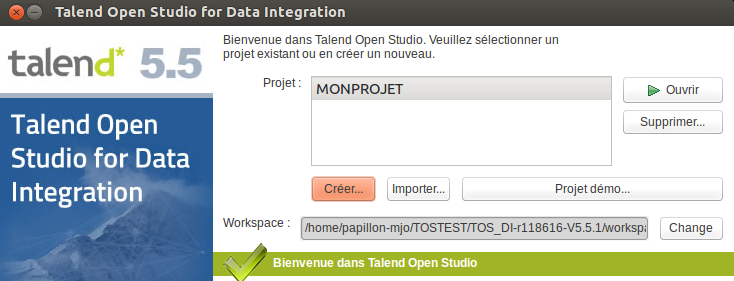
\includegraphics[origin=l,width=13cm]{image/image1.png}	%Ajout d'image

Le workspace du projet est composé des éléments suivants:\\\\
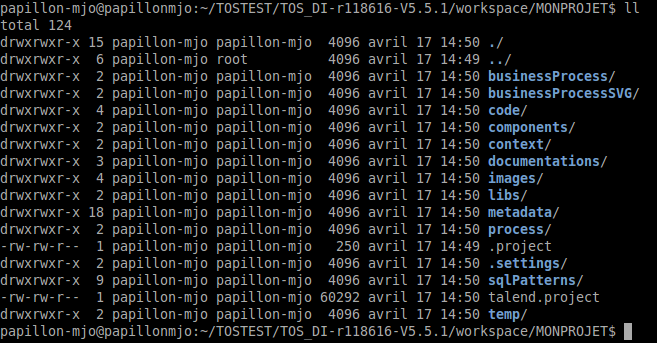
\includegraphics[origin=l,width=12cm]{image/image2.png}

\subsubsection{Initialisation du dépôt git distant}
Sur la machine distante ce placer dans le repertoire contenant vos repos git puis initialiser un nouveau repos:

%Ajout de code
\begin{lstlisting}[language=bash,numbers=left,numberstyle=\tiny,backgroundcolor=\color{Zgris}]		
$ git init --bare MONPROJET.git
\end{lstlisting}

\subsubsection{Initialisation du dépôt git local}

Se placer dans le répertoire du projet puis :

\begin{lstlisting}[language=bash,numbers=left,numberstyle=\tiny,backgroundcolor=\color{Zgris}]
$ git init
\end{lstlisting}

Il suffit ensuite de configurer les fichiers/répertoires qui seront ignorés dans le .gitignore :
\begin{lstlisting}[language=bash,numbers=left,numberstyle=\tiny,backgroundcolor=\color{Zgris}]
sudo vi .gitignore
\end{lstlisting}

ajouter dans le gitignore les éléments suivants:
\begin{lstlisting}[inputencoding=utf8,language=bash,numbers=left,numberstyle=\tiny,backgroundcolor=\color{Zgris},commentstyle=\color{CommentaireGris}]
#Le répertoire temp n'est pas a vérsionner
/temp
#Les routines systèmes sont re-générées à chaque ouverture du projet.
/code/routines/system
#Les patterns SQL sont également re-générées.
/sqlPatterns
*.screenshot
\end{lstlisting}

Ajouter au tracking les éléments suivants:
\begin{lstlisting}[language=bash,numbers=left,numberstyle=\tiny,backgroundcolor=\color{Zgris}]
$ git add .gitignore .project .settings/ talend.project process/
\end{lstlisting}

Commiter les nouveau fichier ajouté :
\begin{lstlisting}[language=bash,numbers=left,numberstyle=\tiny,backgroundcolor=\color{Zgris}]
$ git commit -m "first commit"
\end{lstlisting}

Se connecter au repos distant
\begin{lstlisting}[language=bash,numbers=left,numberstyle=\tiny,backgroundcolor=\color{Zgris}]
$ git remote add origin ssh://@serveur/home/user/MONPROJET.git
\end{lstlisting}

Puis effectuer un push:
\begin{lstlisting}[language=bash,numbers=left,numberstyle=\tiny,backgroundcolor=\color{Zgris}]
$ git push origin master
\end{lstlisting}

Un certain nombre de répertoires sont vides et ne seront donc pas mis en gestion de configuration par git. Cela ne gène pas le bon fonctionnement de l’ensemble. Ajouter les au cour des dev.

Il est en revanche important de commiter le fichier \textbf{talend.project}, afin de permettre l’import du projet par d’autres développeurs.

\subsubsection{Importer et travailler sur le projet}

Plaçons-nous maintenant du point de vue d’un développeur qui compte travailler sur le projet. Il faut tout d’abord cloner le projet dans un répertoire temporaire :

\begin{lstlisting}[language=bash,numbers=left,numberstyle=\tiny,backgroundcolor=\color{Zgris}]
$ mkdir $HOME/tmpMONPROJET
$ cd $HOME/tmpMONPROJET
$ git clone git://gitdistantrepository/talendproject.git
\end{lstlisting}

Ensuite, dans l’écran d’accueil de Talend, il faut choisir Importer le ou les projet(s) existant en local à partir d’un répertoire temporaire que l’on vient de créer.\\\\
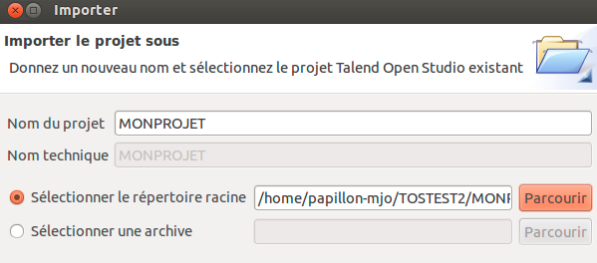
\includegraphics[origin=l,width=10cm]{image/image3.png}

\textbf{Attention : il est important que l’ensemble des développeurs nomment leur projet exactement de la même façon.}

Une fois le projet importé, le répertoire temporaire peut être supprimé. En effet, l’import du projet copie l’intégralité de son contenu, y compris le dépôt git. Dès que le projet est importé, on peut donc travailler directement avec git dans le véritable répertoire du projet.














\end{document}                               % Fin du document
